\chapter{Introduzione}

\section{Differenze tra relational/non-relational DB}
Lorem ipsum dolor sit amet, consectetur adipiscing elit. Suspendisse et ex vehicula, interdum mi eu, auctor augue. Suspendisse vel sagittis urna. In vitae ligula ipsum. Vivamus mattis neque efficitur, gravida purus facilisis, rhoncus felis. Class aptent taciti sociosqu ad litora torquent per conubia nostra, per inceptos himenaeos. Nunc bibendum urna porta quam congue ornare. Fusce eget consequat libero. Donec varius justo vel libero malesuada, sit amet dignissim ex tincidunt. In pharetra vestibulum lacus quis laoreet. Donec vel laoreet ex, sed facilisis massa. Mauris commodo velit est. Maecenas non sem elementum, faucibus velit et, bibendum mi. Integer laoreet ex et eros accumsan, nec dapibus nisi vestibulum. Donec sed nunc quis mi gravida congue non vel tortor. Interdum et malesuada fames ac ante ipsum primis in faucibus.

Nullam non pharetra arcu. Donec eget velit elit. Pellentesque sed tortor sodales neque tristique rutrum. Vivamus et ex dolor. Vestibulum lacinia augue sit amet libero mattis pellentesque. In sed congue ante, quis tempus neque. Vestibulum semper eu sapien et vestibulum.

In ac erat ullamcorper, ultricies dolor sit amet, tempus neque. Pellentesque quam erat, ornare ac justo at, cursus luctus ex. Pellentesque at turpis blandit, elementum ex ac, fringilla nibh. Etiam et tincidunt lacus. Integer mattis mi sit amet faucibus rutrum. Sed at nisi commodo, ultricies purus a, tempus lacus. Mauris accumsan enim nisi, in tempor velit pharetra eu. Sed eu turpis et ante sagittis sodales. Duis a tellus id risus ultricies accumsan. Vestibulum bibendum in sapien sit amet rhoncus. Fusce aliquam, metus vel efficitur pulvinar, nibh lacus ultricies nisl, nec rhoncus elit ligula vitae risus. Mauris bibendum eget erat non rutrum. Curabitur in ligula eget lectus facilisis molestie sed sed neque. Vestibulum eu faucibus augue, a luctus augue. Nam lobortis massa non lorem condimentum vehicula. Aliquam efficitur cursus neque, efficitur placerat libero tincidunt non. Nullam.


\section{Il nostro caso di studio}

Durante la progettazione si e' deciso di utilizzare una relazione per poter testare i diversi metodi di collezione dei dati.
La relazione e' formata da 2 entita' A e B,in un esempio di un social network l'entita' A sono i Post e l'entita' B i Commenti sotto ogni post, collegate da una relazione 1..N,
per ogni A esistono 10 B relativi, ogni Post contiene 10 Commenti.

La modellazione delle entita' e' stata fatta creando 2 triplette di attributi uguali, sulla seconda tripletta al contrario della prima sono stati costruiti degli indici su ogni attributo,
questi attributi generici hanno una propria selettivita':

    \begin{equation*}
        \left.\begin{aligned}
         sel(Att1, Att4) &= \frac{1}{10}    \\
         sel(Att2, Att5) &= \frac{1}{10.000} \\
         sel(Att2, Att6) &= \frac{1}{100}
        \end{aligned}
        \right\}
        \qquad 
        \end{equation*}

Poi un attributo testaule di 100 bytes per poter inserire descrizione.

Il numero di Entita' A e' di $10^5$ e di conseguenza ci sono $10^6$ entita' B.

!!!!!!!!!! LE FOTO NON VANNO BENE, LE CHIAVI DEVONO ESSERE SEGNALATE !!!!!!!!!!!!!!!!!!!!!!!!!
\begin{center}
    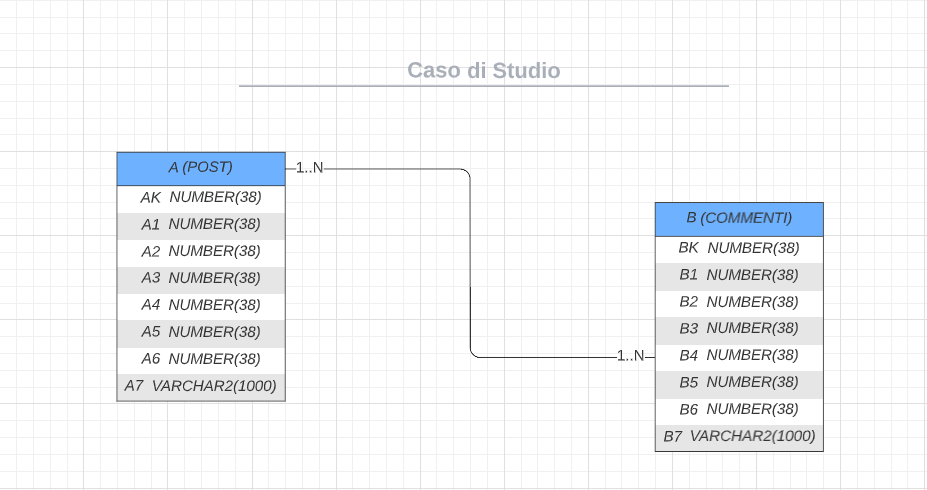
\includegraphics[scale=0.6]{Caso Studio.png}
\end{center}


\section{Modellazione dei dati}

La modellazione dei dati ha un ruolo fondamentale nel calcolo dei costi di accesso e quindi costi di esecuzione delle query, le soluzioni dalle quali si e' deciso di di partire 
sono quelle dell'Embedding e del Referencing. Utilizzando un sistema non relazionale abbiamo necessita' di esprimere la relazione tra A e B in un modo differente, attraverso il 
referencing colleghiamo le un entita' inserendo un riferimento della seconda e viceversa, per poter poi eseguire ad esempio query di join o voler recuperare tutti i dati 
dell'entita' referenziata c'e' il bisogno di mantenere all'interno del database la collezione contenente i rimanenti attributi. Es. nell'eventuale soluzione del referencing di B all'interno 
di A, ci sono due collezioni ossia A con la foreign key relativa (BK) relativa a B e l'intera collezione B. 

\begin{center}
    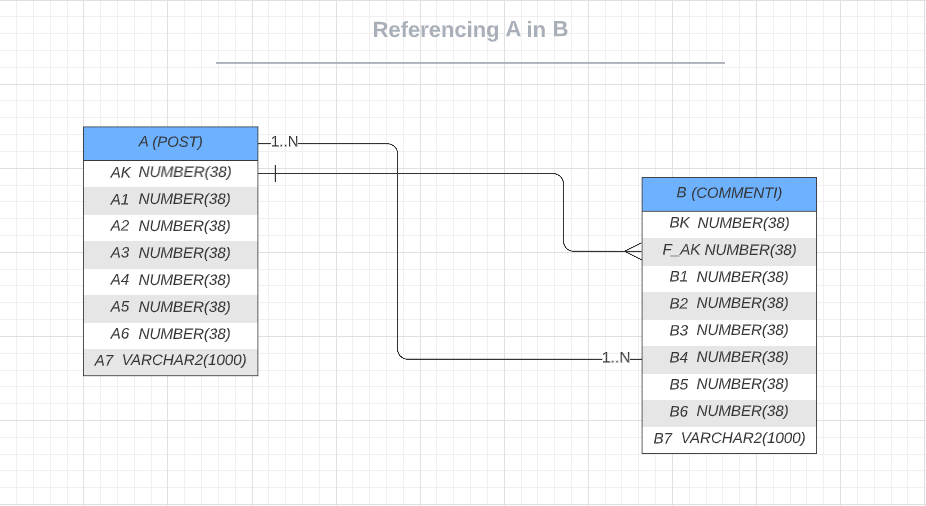
\includegraphics[scale=0.6]{refAB.png}
\end{center}

\begin{center}
    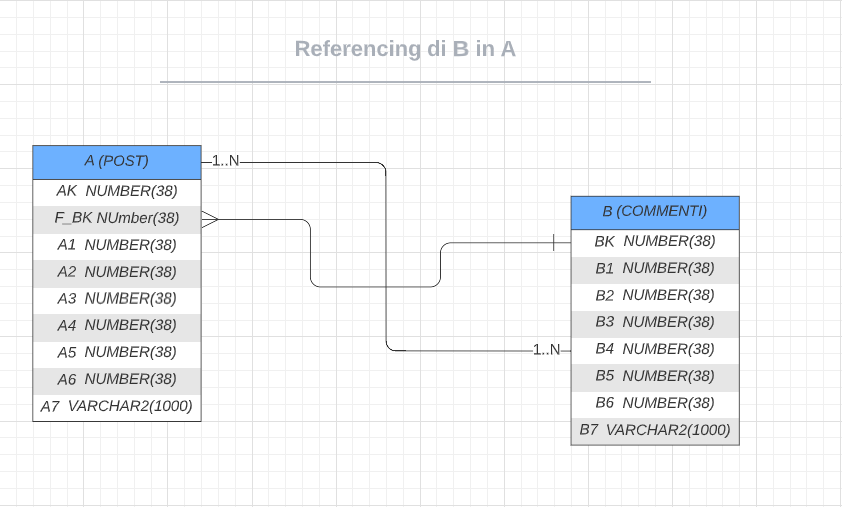
\includegraphics[scale=0.6]{refBA.png}
\end{center}

La soluzione embedding consiste nel creare un'unica collezione di documenti che racchiudono al loro interno sia documenti di A che documenti di B.

\begin{center}
    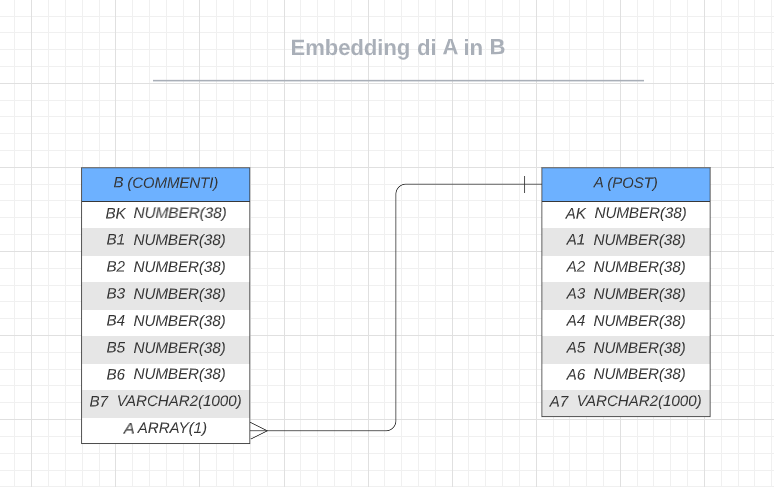
\includegraphics[scale=0.6]{embAB.png}
\end{center}

\begin{center}
    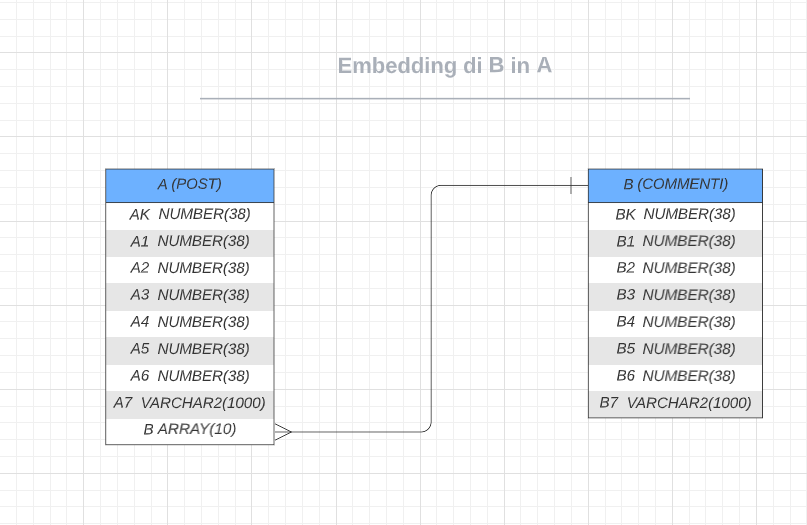
\includegraphics[scale=0.6]{embBA.png}
\end{center}
